\documentclass{article}
\usepackage[utf8]{inputenc}
\usepackage{graphicx}
\usepackage{color}

\newenvironment{text-blue}{\color{blue}}{}
\newenvironment{text-red}{\color{red}}{}

\begin{document}

\title{Classificação de ruído em biosinais \\ Trabalho prático nº2, Computação Adaptativa}
\author{Adriano Vinhas (2009106560, avinhas@student.dei.uc.pt)\\
		José Ribeiro (2008112181, jbaia@student.dei.uc.pt}
\maketitle
\clearpage

% Introdução
\section{Introdução}

\indent \indent Este trabalho, no âmbito da disciplina de Computação Adaptativa, tem como objectivo construir uma rede neuronal multimacamada capaz de reconhecer se um sinal biológico deve ser descartado (devido à presença de ruído) ou deve ser analisado. Este reconhecimento é feito com base num conjunto de características do sinal que vão servir de entrada para a rede neuronal.

Este objectivo foi atingido fazendo um estudo paramétrico tendo em conta os seguintes parâmetros de estudo:
\begin{itemize}
\item Método de treino
\item Coeficiente de aprendizagem
\item Número de neurónios na camada escondida
\item Dimensionalidade do problema
\item Número de épocas do treino
\item Aplicação de normalização sobre os dados
%\item Goal (Erro de treino) ???
\end{itemize}

A parte que foi mais focada na realização deste trabalho foi o estudo paramétrico feito com base nos parâmetros acima indicados. Com base nos resultados obtidos, procurámos uma solução que nos permitisse chegar à combinação dos parâmetros que optimizasse os valores de sensibilidade e especificidade das saídas da rede.

\clearpage
\section{Concepção da rede neuronal}
\indent \indent Nesta secção estão descritas a arquitectura da rede usada para o trabalho e a forma como foi feito o treino da rede.

A arquitectura da rede neuronal usada para o trabalho prático caracteriza-se por 26 entradas e 1 saída, sendo que cada uma das entradas representa uma característica do \textit{dataset} que nos foi fornecido e a saída representa a decisão (se o sinal deve ser descartado ou analisado). No entanto, para os testes efectuados, o número de entradas da rede está sujeito a alterações, sendo este número dependente do uso (ou não) de mecanismos de redução de dimensionalidade.

A função de activação usada para a camada interna foi a tangente hiperbólica, para garantir que a rede neuronal pudesse ser um aproximador universal, e para a camada de saída foi usada uma função linear.

A figura~\ref{nn_architecture} representa a arquitectura da rede usada.

\begin{figure}[!h]
  \centering
  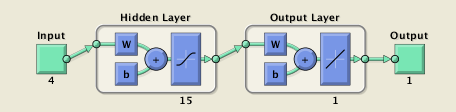
\includegraphics[width=3in]{figures/nn_architecture}
  \caption{Arquitectura da rede usada (com 26 características e 15 neurónios na camada escondida)}
  \label{nn_architecture}
\end{figure}

O \textit{dataset} usado para este trabalho é composto por um total de 12331 exemplos. Deste conjunto, 70\% dos exemplos (8632) foram usados para treinar a rede, e os restantes 30\% (3699) para validação desta e análise de resultados.

O método de selecção de exemplos para cada um dos conjuntos é aleatório. Para que tal aconteça, todos os exemplos são "baralhados" e ficam dispostos numa ordem completamente à ordem original. De seguida é feita a separação segundo a regra 70/30, tal como enunciado acima.

\clearpage
% Gráficos com os resultados. Análise e interpretação.
\section{Estudo paramétrico}
\indent \indent Nesta secção são apresentados os resultados do estudo paramétrico efectuado para obtenção do resultado óptimo encontrado.

De forma a analisar a performance de ambas as abordagens sob diferentes subconjuntos de padrões, 30 subconjuntos distintos de padrões de treino e validação foram gerados. Os erros cometidos na fase de validação por ambas as abordagens quando submetidas ao treino sobre esses subconjuntos foram contabilizados ao longo das 30 execuções. Os resultados obtidos são evidenciados na figura~\ref{nn_long_run_performance}, onde se apresenta a performance média de cada abordagem ao longo das 30 execuções.



Num total de 1170 classificações\footnote{1170 classificações: 3 classificações por cada um dos 13 dígitos, ao longo de 30 execuções.}, o \textbf{Perceptrão} obteve um total de \textbf{176 classificações incorrectas}, enquanto que a \textbf{Memória Associativa Linear} obteve \textbf{139}; tais resultados correspondem a taxas de eficácia de \textbf{84.96\%} e \textbf{88.12\%}, respectivamente.

A \textbf{Memória Associativa Linear} obteve, assim, uma \textbf{performance média ligeiramente superior} à do Perceptrão na resolução deste problema, considerando os conjuntos de padrões de treino e validação utilizados.

A superioridade de 4\% pode ser justificada pela capacidade de \textbf{tolerância} e \textbf{correcção} de padrões com ruído que um Perceptrão não apresenta; essa capacidade permite que os desvios naturais do dígito protótipo possam ser ignorados de forma a obter, ainda assim, a classificação correcta.

É de notar que a distância de \textit{Hamming} entre os padrões de dígitos perfeitos de símbolos como \texttt{2}, \texttt{5} e \texttt{8} é bastante pequena quando comparada com o número de entradas (tão pequena quanto \textbf{2 entradas diferentes num espaço de 25 entradas}). Tal facto torna o conjunto de dados de treino e validação extremamente importante no que toca à aprendizagem da rede neuronal da relevância e crucialidade de certas entradas para a correcta identificação dos dígitos. É também notório que o \textbf{reduzido espaço de estados} (e consequente proximidade entre dígitos válidos) torna a correcta aprendizagem da rede mais difícil (pelo facto anteriormente mencionado), pelo que julgamos que a classificação beneficiaria de um \textbf{mais alargado conjunto de entradas} (dígitos de 7x5, por exemplo).

\clearpage
\section{Conclusão}
\indent \indent Depois do estudo paramétrico efectuado a rede neuronal que obteve melhores resultados tinha um valor de sensibilidade de \begin{text-red}\textbf{xx.xx\%}\end{text-red} e de especificidade igual a \begin{text-red}\textbf{xx.xx\%}\end{text-red}.

Atingimos estes valores usando a seguinte parametrização:
\begin{itemize}
\item Método de treino: \texttt{trainlm} (Levenberg-Marquardt)
\item Coeficiente de aprendizagem: Não aplicável
\item Número de neurónios na camada escondida: \begin{text-red}x\end{text-red}
\item Dimensionalidade do problema: \begin{text-red}x\end{text-red}
\item Número de épocas do treino: \begin{text-red}x\end{text-red}
\item Aplicação de normalização sobre os dados: Sim
%\item Goal (Erro de treino) ???
\end{itemize}

\end{document}
